\chapter{Background}
\label{chap:background}

In the following, first the preliminary information about crowdsourcing concepts 
is summarized, since crowdsourcing is a relatively area of computation. Later,
the building blocks of a crowdsourcing platform are described, and related studies 
are examined thoroughly over this description.

\section{Preliminaries}
Crowdsourcing term is first proposed by Jeff Howe~\cite{Howe2006b} in 2006. 
Although there is a long list of terms (collective intelligence, social computing, 
human computation, global brain etc.), in which some of them are new and some 
others are old, the use of term "crowdsourcing" in the academia (demonstrated in 
Figure~\ref{fig:keywordstats}) indicates that research on this domain is promisingly 
increasing.

\begin{figure}[ht]
	\centering
	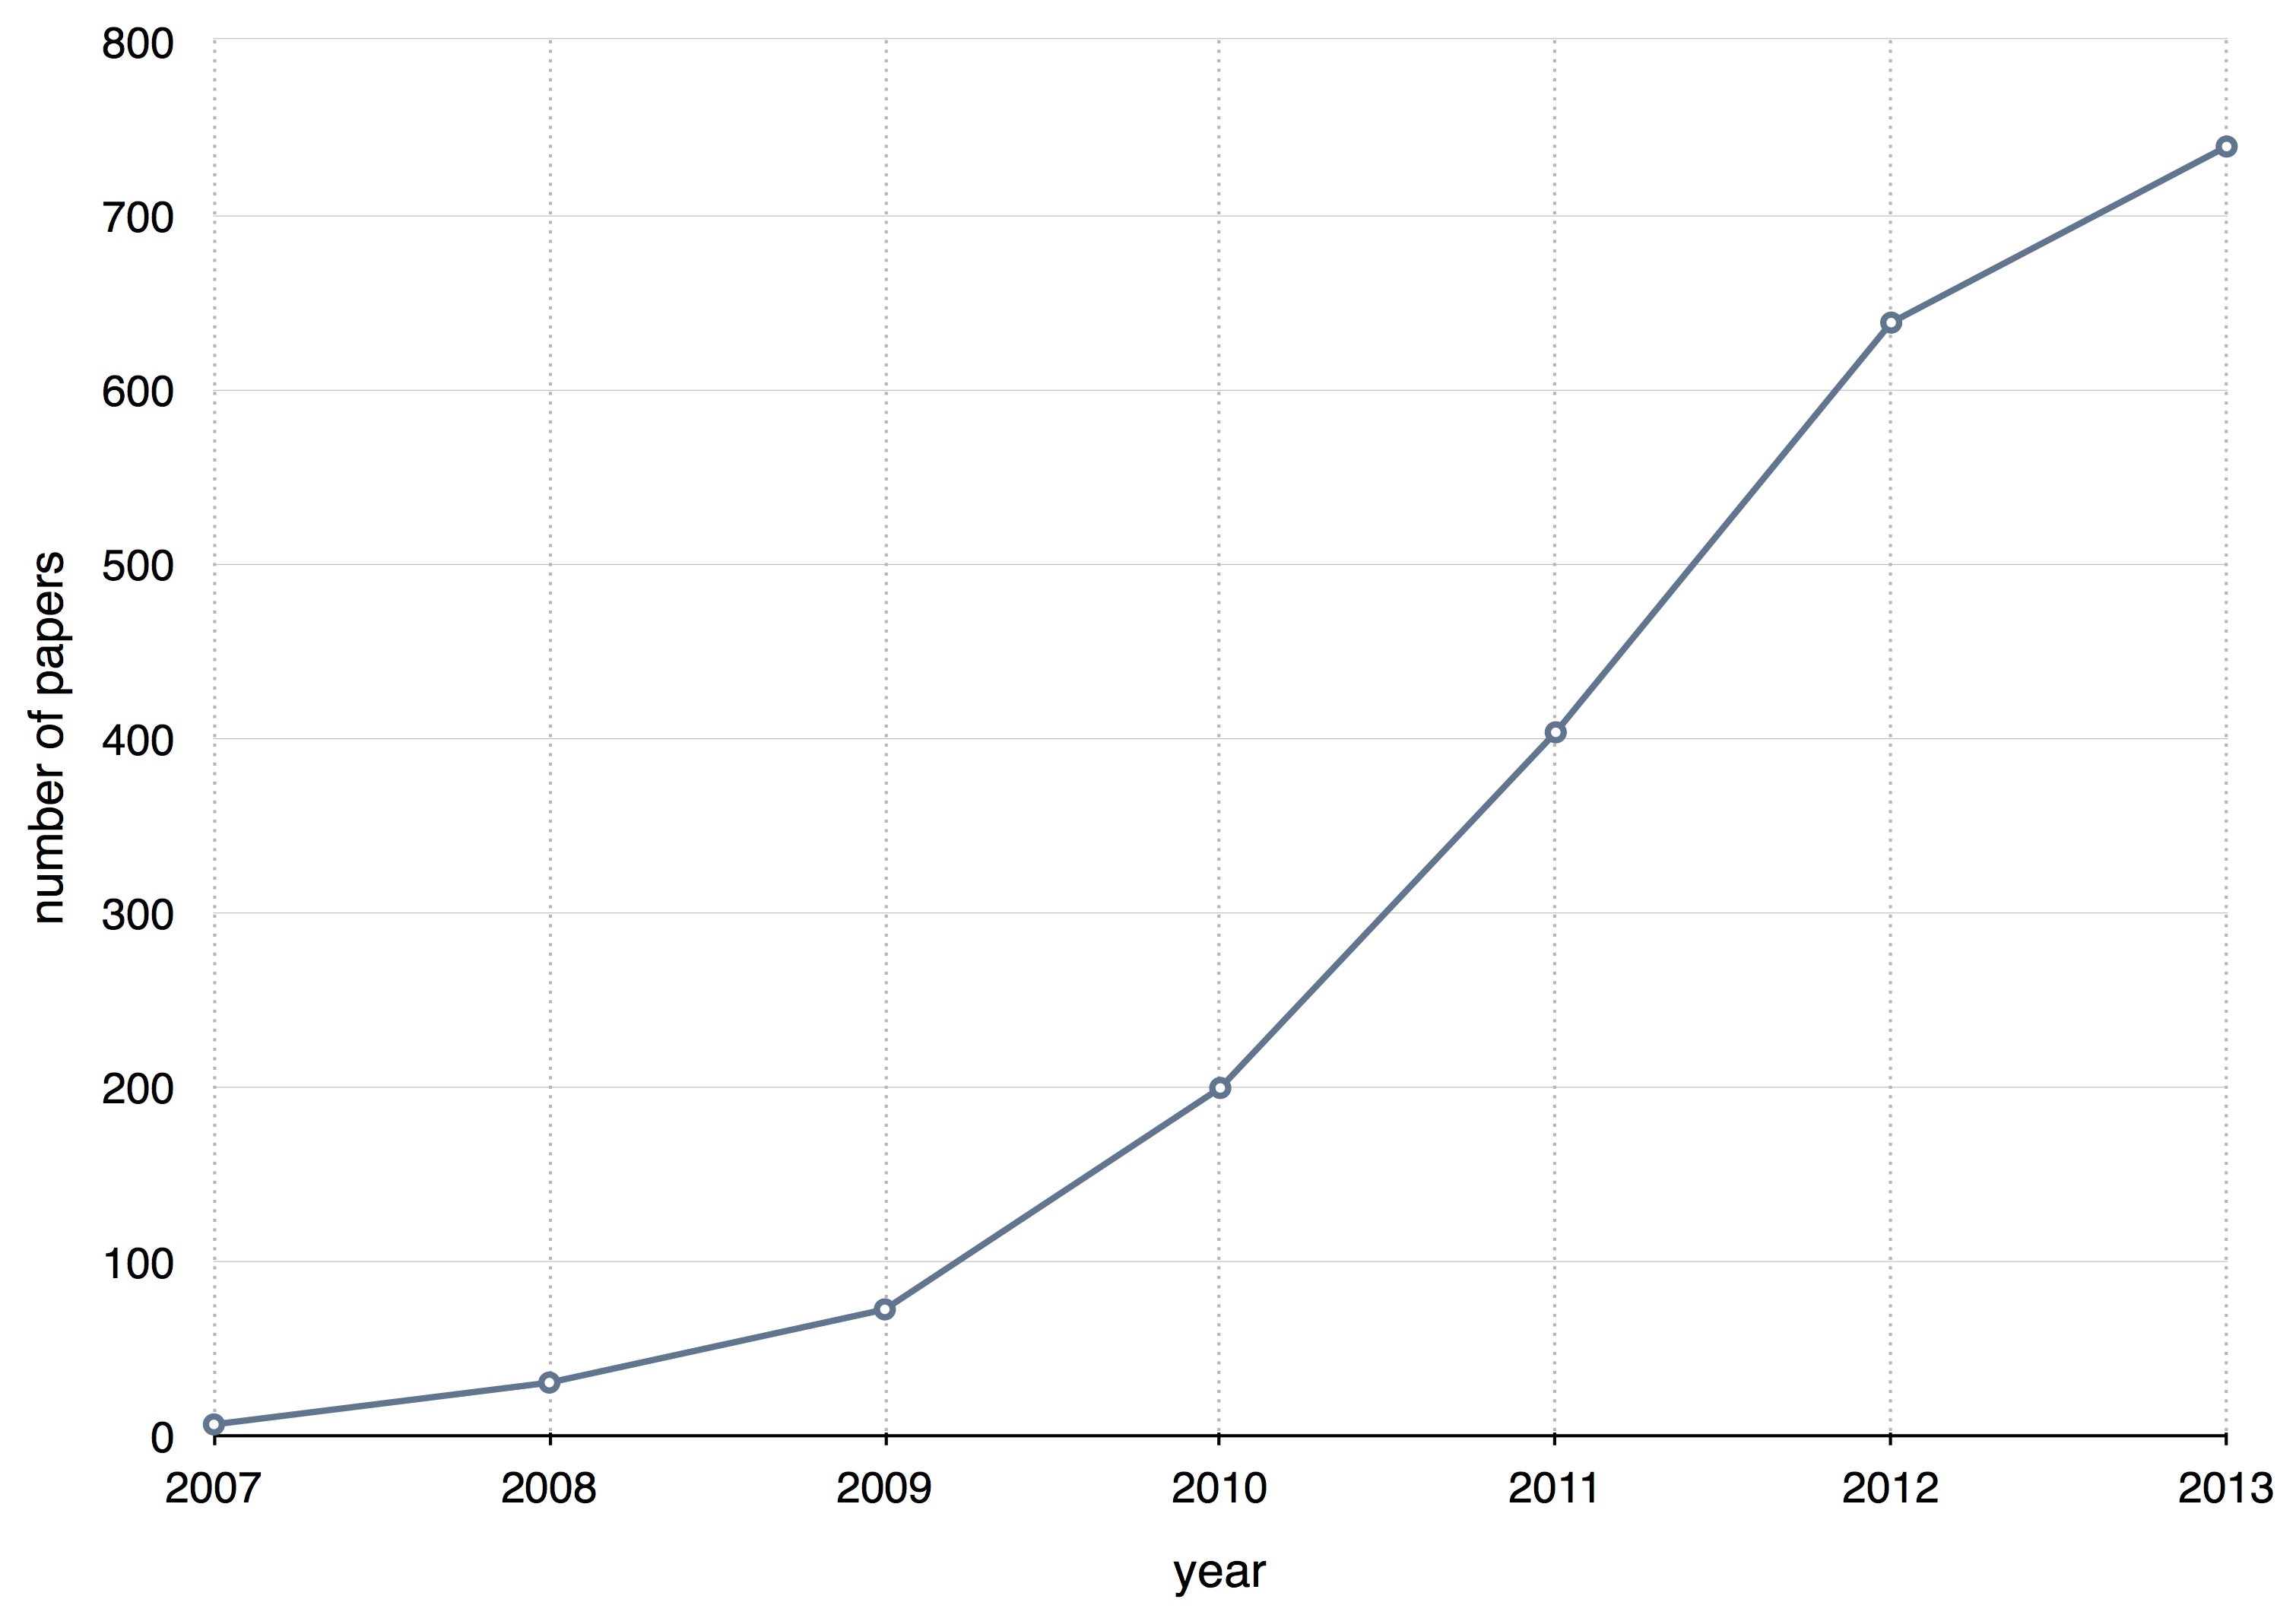
\includegraphics[width=0.85\textwidth]{figures/keyword_statistics.png}
	\caption[The frequency of crowdsourcing keyword in academic papers.]{The frequency of crowdsourcing keyword in academic papers.\footnotemark}
	\label{fig:keywordstats}
\end{figure}

Researchers have been exploring different approaches to employ crowd of people 
in solving various problems. From task creation to quality control there has been a 
lot of research in crowdsourcing.  In most of these studies, Amazon's Mechanical 
Turk (MTurk) is the main consideration on crowdsourcing where new proposals are 
implemented and executed on this platform. MTurk is an 
intermediary platform between employers (known as requesters) 
and employees (workers or turkers) for various-sized and difficulty assignments. 
The platform has become successful for tackling the problems that cannot be 
solved by computers and subject to numerous research studies.

Similar to other academic studies, MTurk is considered in this work to discuss 
the common terms and form a preliminary list of concepts. In the following, 
the fundamental concepts of crowdsourcing is explained.

\footnotetext{The statistics are gathered through ACM Digital Library.}

\subsection{Tasks}
Task is a piece of work to be done by the crowd. Terms task, micro-task and job 
are interchangeably used. The term Human Intelligent Task or HIT is commonly 
used as well. A task is often expressed over an HTML form in which there are three 
different input types: single selection (radio buttons), multiple selection (checkboxes) 
and free text (text areas). For single and multiple selection one or more items can be 
selected from a list of possible options. Considering free text types workers are 
supposed to enter a textual response that can be paragraph(s) or sentence(s) 
or number(s).

In addition to the labels attached to input forms, task has a short description 
that provides the instructions and keywords, which will help workers search for 
specific tasks. Further, number of assignments (copies) that requester wants completed 
per task can be set. Additional copies of the same task allows parallel processing. 
In that case, the system is supposed to ensure that the parallel workers are unique 
(i.e., no single worker complete the same task more than once).

A task is generally simple requiring small amount of time and expertise to complete. 
In the following, sample tasks from MTurk are presented.

[Sample Tasks Figure Will Come Here]

Tasks can be grouped into task groups. Task groups are for the tasks that share 
similar qualities such as tasks to tag images of nature and people or tasks asking
for translation of a text snippet from a language to another.

\subsubsection{Time}
Often time scale requiring to complete a task ranges from seconds to minutes. 
Nearly 20\% of tasks takes less than 1-hour, and more than half of tasks does not 
take more than 16-hours~\cite{Ipeirotis2010}. Maximum time allotted per 
assignment can be set by requester. 

\subsubsection{Payment}
Compensation or reward for completing tasks range from a single penny to dollars. 
An analysis of MTurk showed that 90\% of tasks pays \$0.10 or less~\cite{Ipeirotis2010}.

\subsubsection{Acceptance}
Once a worker completes and submits an assignment, the requester is notified. 
The requester has an option to either accept or reject the completed assignment. 
Acceptance of an assignment, which indicates the work done is satisfactory, 
makes the worker who completed it get paid, on the other hand rejection withholds 
payment for which the reasoning may or may not be provided by the requester. 
Another option is automatic approval, which is the case when requester does not 
review work after a some time that can be set by the requester.

\subsubsection{Expiration}
Tasks have a lifetime limit that decides the amount of time that a particular task 
remains in the listings. Lifetime can be set by requester. After a task reaches 
end of its lifetime, it is automatically pulled from the listings.

Another type of expiration can happen while a worker is operating on an assignment. 
When workers accept an assignment, the assignment is reserved for them making 
no other worker to accept it. The reservation is for particular piece of work 
(in this case assignment) and time-limited. If worker does not submit the completed 
assignment in allotted time, then reservation is cancelled and assignment is 
made available for others again.

\subsection{Requesters}
Requesters are the employers who post tasks, obtain results and pay workers. 
Requesters are expected to design tasks with all the details (description, instructions, 
question types, payment, expiration settings etc.) After completed assignments 
are submitted, requesters can review them by accepting or rejecting, 
and collect the completed work. 

These operations can be done via user interface or application programming 
interface (API) if there is one. 

\subsection{Workers}
Workers are the online users or someone from the crowd who work on and 
complete assignments in exchange for a small payment. On some platforms 
(currently not available on MTurk), detailed information about workers are gathered 
and kept in a database. This information can be later utilized by requesters while 
associating specific constraints to the assignments such as limiting age to some 
range for a specific task. 



\section{Building Blocks of a Platform}
Kittur et al. provides a detailed description for the future crowdsourcing platform 
in~\cite{Kittur2013}. Based on this description building blocks of a crowdsourcing 
platform is defined in the following.

A crowdsourcing platform is a platform to manage tasks and workers in the 
process of solving problems through multi-stage workflows. Platform should enable 
decomposition of complex tasks into subtasks and assign them appropriate group of 
workers. Workers are formed by people with different skills and expertise. The motivation 
of workers is guaranteed through various approaches 
such as reputation or payment. Quality assurance is required to ensure the output 
of a task is high quality and contributes to solution.

Regarding this definition, a crowdsourcing platform consists of three basic elements:

\subsection{Workflow Design}
Complex and sophisticated problems cannot be solved by current simple parallel 
approach. The reason is that these problems have interdependent portions with 
changing space, time and skill-set requirements. On the other hand, current 
approaches undertake problems through bulk processing of independent 
and simple tasks that require no specific expertise. Therefore, a more appropriate 
problem solving approach is required.

The need for a more advanced approach is mentioned in \cite{Kittur2013}. Authors 
indicate $workflows$ in the sense of decomposing problems into smaller chunks, 
coordinating dependencies among these chunks and combining results from them. 
In that sense, workflow design refers to the development of applications to solve 
complex problems. It considers design and management of computation resources 
to solve the problem.

Researchers often apply existing programming paradigms to problem specification 
and workflow design. MapReduce~\cite{Kittur2011, Ahmad2011}, 
Divide-and-Conquer~\cite{Kulkarni2012}, 
Iterative~\cite{Little2009}, 
Workflow ~\cite{Kokciyan2012} are some of these approaches taken for 
organizing and managing complex workflows. Although these paradigms 
perfectly fit to some problems, there are other problems not suited well to those. 

In terms of crowdsourcing, workflow could involve different scale of operations that 
can only be solved by diverse set of actors. A workflow may tackle highly dependent 
tasks (e.g., translating a poem and assuring its quality) or massively parallel 
tasks (e.g., finding some piece of information on the Web). Therefore, the workflow 
design has diverse space requirements.

\subsection{Task Assignment}
In the context of crowd work, coordination of limited resources is prominent, 
because problems has various types of tasks that require coordination and 
collaboration of different computation resources. Crowdsourcing problems  
have pieces that cannot be computerized, but require human intelligence. In 
addition, there may be other problems that require both human and software 
resources.

Although availability and assignment of software resources can be managed 
by certain algorithms, the case for human resources is rather unpredictable and 
hard to solve. Human resources are formed by workers and the availability of a 
worker cannot be predicted or known at any time. In fact, human resources 
are not homogenous like computers. They are rather heterogeneous and each 
worker in the crowd has a specific set of skills. Therefore, there may be a situation 
in which a task couldn't be assigned to any available workers due to mismatch 
between task's requirements and skill-set of available workers. Ideally workers 
are employed with tasks that fit their area of expertise. In practice, requesters 
may disregard this constraint, but results would not be useful at all.

One important point is that existing systems are misleading by assuming 
human crowd is homogeneous. Task assignment needs to be redefined 
by demonstrating aspects of human resources.

\subsection{Quality Control}
Quality control is a big challenge for crowdsourcing platforms, since low quality work 
is common. It is shown that low quality submissions can compromise up to one third 
of all submissions~\cite{Bernstein2010}. As a result, researchers have started to 
investigate several ways of detecting and correcting for low quality work.

Visualization of workflow is one of the methods employed for which directed graphs 
are used to show the organization of crowdsourcing tasks, allowing endusers 
to better understand the problem and proposed solution design~\cite{Kulkarni2012, Kittur2012}.

Inserting 'gold standard' questions into an assignment by which workers 
who answer them incorrectly can be filtered out or given feedback~\cite{Burch2009}. 
However, writing validation questions create extra burden to requesters and 
may not be applied to all types of tasks.

Majority voting to identify good submissions is proposed as another 
option~\cite{Burch2009, Bernstein2010}, but this technique can be affected 
by majority (especially when the possible options are constrained) or failed in 
situations where there are no answers in common such as creative or generative 
work~\cite{Rzeszotarski2012}.

Systems (including MTurk) often do not apply any of these quality control approaches, 
but provide other ways to achieve good workers and discourage bad ones. 
Currently each worker on MTurk has an acceptance rate that is updated after 
requester's review on completed assignments. However, this feature does not 
differentiate one type of task from the other in terms of effect on acceptance rates 
and that makes it a limited utility. A worker who is skilled in audio transcription would 
probably have high accuracy rating in related tasks. However, there is no way to 
reason that this worker can also perform English-to-Turkish translation tasks. 
Even worse is that workers who pick and complete easy tasks would probably 
have higher accuracy rates than the ones who choose to perform tasks that 
require time and expertise~\cite{Barowy2012}.

Requesters can utilize acceptance rates by assigning a low limit of them to 
assignments, which allow only workers with acceptance rates above-limit 
to accept assignments.
